\chapter{Governing Equations} \label{chap:governing-equations}
\section{Single Particle Motion Along Magnetic Field Line}
The motion of charged particles in magnetic field is determined by the magnetic force,
\[ m\dv{\mathbf{v}}{t} = q\mathbf{v\times B} \]
where $m$ is the mass of charged particle, and $q$ is the charge of particles.

Consider a magnetic field pointing in z-direction, $\mathbf{B}=B\mathbf{\hat{z}}$. Since the magnetic force is perpendicular to both $\mathbf{v}$ and $\mathbf{B}$, we can separate the equation of motion into two directions,
\[ 
q\mathbf{v_{\perp}\times B} = \frac{mv_{\perp}^2}{r}\mathbf{\hat{r}}, 
\quad
\mathbf{v}_{\parallel} = v_{\parallel} \mathbf{\hat{z}} \]
where $\mathbf{v}_{\perp}$ is the velocity perpendicular to the magnetic field, and $\mathbf{v}_{\parallel}$ is the velocity parallel to the magnetic field. In this way, we see that the charged particle gyrates about the magnetic field, doing helical motion along the magnetic field line. 

Moreover, if we assume a static, nonuniform $\mathbf{B}$ field, the particles will stay on the same magnetic field line due to the so-called longitudinal invariant 
\[J = \int_{a}^{b} v_{\parallel} ds\]
where $[a,b]$ is the region of magnetic nozzle.  
\begin{figure}[H]
	\centering
	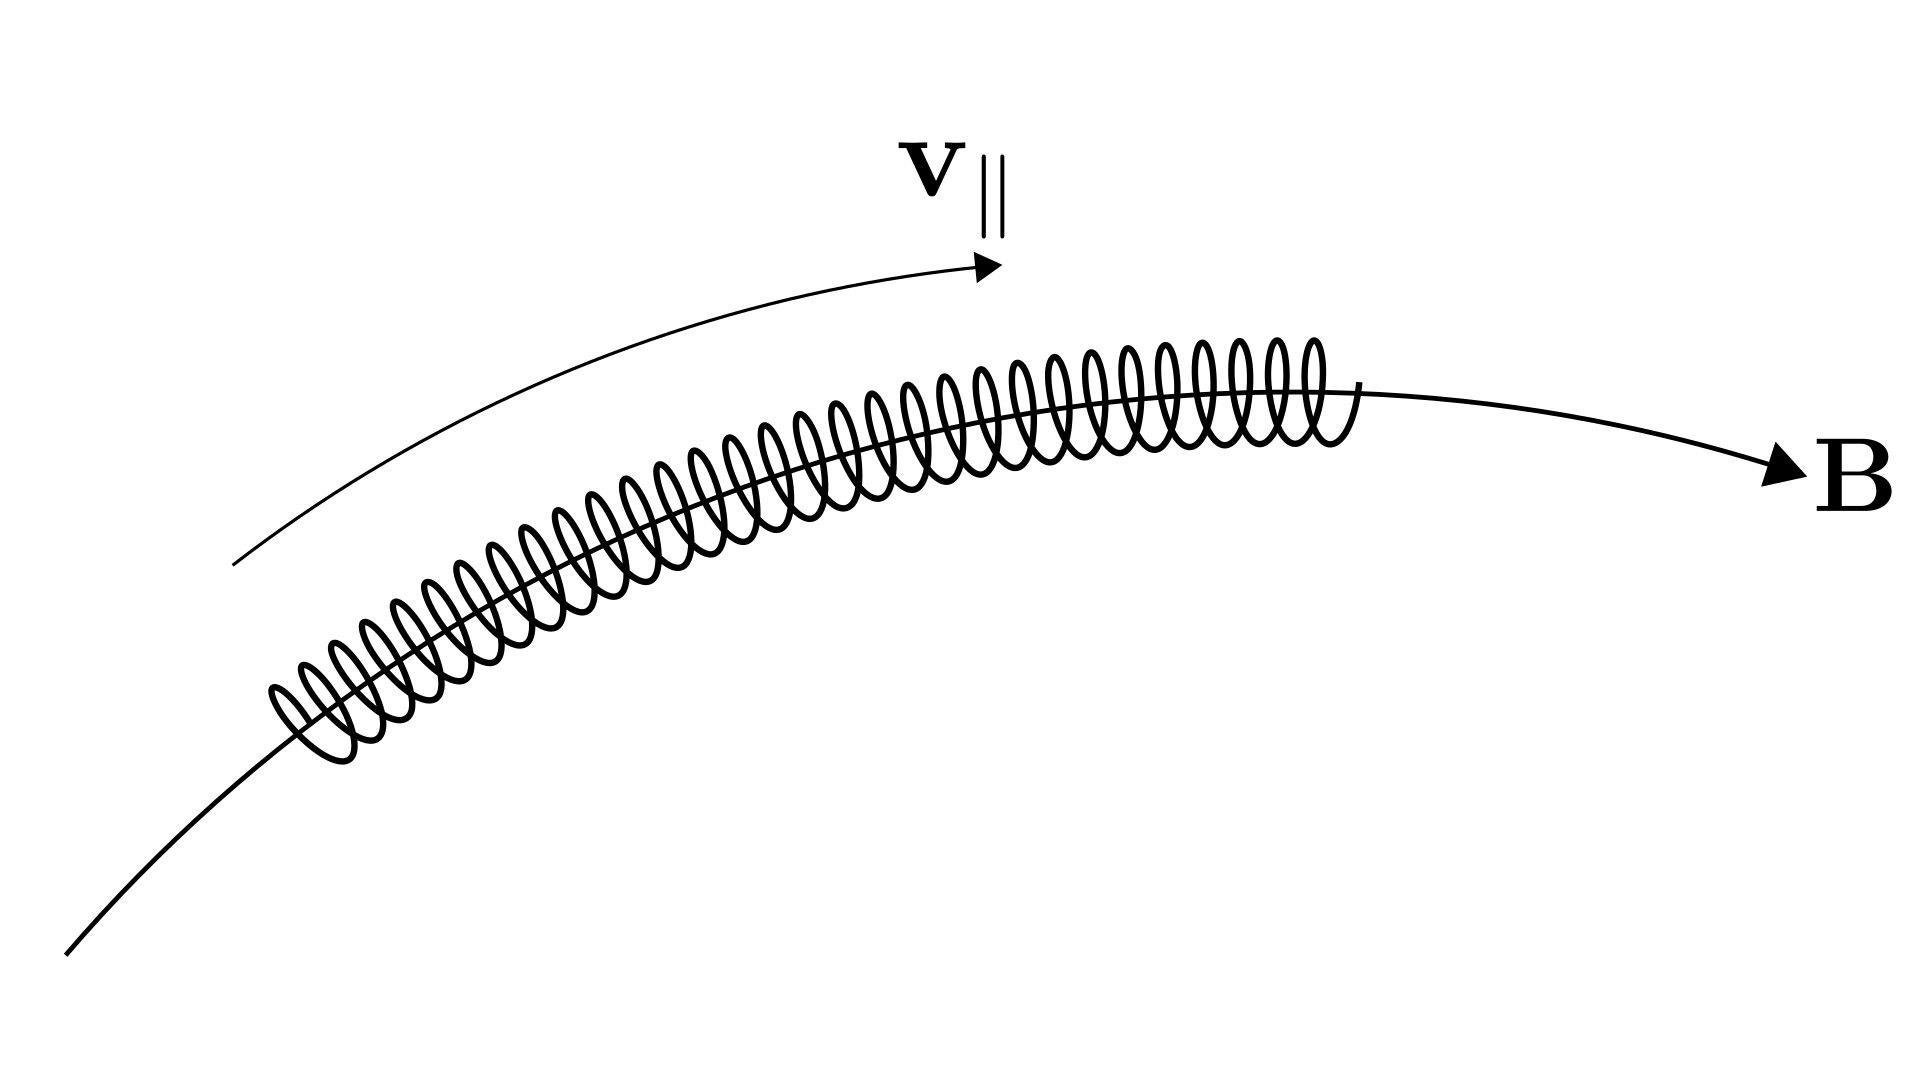
\includegraphics[width=0.7\linewidth]{img/governing-equations/gyrate-along-b-field}
	\caption{A charged particle gyrates about the magnetic field line. The velocity along the field line is $\mathbf{v}_{\parallel}$ and the gyrate frequency, radius is given by the radial equation, $q\mathbf{v_{\perp}\times B} = \mathbf{\hat{r}} mv_\perp^2/r$. Moreover, for static, nonuniform magnetic field, the charged particle will stay on the same of magnetic field line as it gyrates.}
	\label{fig:gyrate-along-b-field}
\end{figure}


\section{From Kinetic Theory to Fluid Description}
In kinetic theory, the charged particles in plasma obey a certain distribution function $f(\mathbf{x}, \mathbf{v}, t)$. This distribution function is affected by plasma temperature. Assuming there is only one species of particles in the plasma, the plasma temperature is just the sum of the kinetic energy of all particles. We expect at higher temperature, faster the particles will be.

At equilibrium, the particles can be characterized by Maxwell-Boltzmann distribution
\[ f_M(\mathbf{x}, \mathbf{v}, t) = \frac{1}{(\pi v_{th}^2)^{3/2}} \exp(-\left(\frac{v}{v_{th}}\right)^2) \]
where $v_{th} = \sqrt{2k_BT/m}$ is the thermal velocity.

The moments of the distribution function are suitable macroscopic properties of the plasma. For example, the plasma density and plasma momentum can be viewed as 
\[ n(\mathbf{x}, t) = \int_{\mathbb{R}^3} f(\mathbf{x}, \mathbf{v}, t) d^3\mathbf{v} \]
\[ n\mathbf{V}(\mathbf{x}, t) = \int_{\mathbb{R}^3} \mathbf{v}f(\mathbf{x}, \mathbf{v}, t) d^3\mathbf{v} \]
where $\mathbf{V}$ is the fluid velocity of the charged particle. It is the bulk velocity of the plasma. In magnetic nozzle, since the charged particles flow along the magnetic field line, it is intuitive to think of $\mathbf{V}$ as the plasma flow velocity along the magnetic field line.

In fusion device and space propulsion system, we want high plasma temperature to achieve good performance. Hence, we assume high plasma temperature in this thesis. In other words, the plasma is collisionless. 

The distribution function $f$ in a collisionless plasma satisfies the so-called collisionless Vlasov equation, $\dv*{t} f(\mathbf{x}, \mathbf{v}, t) = 0$. Expand it explicitly, it is
\begin{equation} \label{eq:vlasov}
	\pdv{f}{t} + \mathbf{v}\pdv{f}{\mathbf{x}} + \frac{q}{m}(\mathbf{E} + \mathbf{v}\times\mathbf{B})\pdv{f}{\mathbf{v}} = 0
\end{equation}
where $q(\mathbf{E} + \mathbf{v}\times\mathbf{B})$ is the Lorentz force experience by the species, the collision term $C(f)$ is dropped. Worth to mention that the electric field and magnetic field are generated by the configuration and the motion of the charged particles.

Integrate both sides with respect to volume element in velocity space, $d^3\mathbf{v}$, we get the conservation of density.
\[ \pdv{\rho}{t} + \div(\rho\mathbf{V}) = 0 \]

If we multiply $\mathbf{v}$ on both sides and integrate with respect to $d^3\mathbf{v}$, we get the conservation of momentum.
\[ \rho\pdv{\mathbf{V}}{t} + \mathbf{V}\cdot\grad{\mathbf{V}} = \frac{q}{m}(\mathbf{E+V\times B}) - \grad{p} \]
In the process we assume isotropic pressure, and no viscosity exists in the plasma.

As we can see the fluid description only depends on the macroscopic properties of plasma, such as the fluid velocity along the magnetic field line $\mathbf{V}$, density $\rho$, and pressure $p$ of the plasma. This simplifies the problem.

\section{Governing Equations for Flow in Magnetic Nozzle}
In this section, we will derive the governing equations of the flow in magnetic nozzle, starting from the fluid description for plasma.

In magnetic nozzle, the magnetic field is along the nozzle, which we denote as z-axis. Due to Lorentz force, the charged particles gyrates about the magnetic field lines. Because the magnetic moment is invariant in such situation (\textbf{reference}). The fluid velocity of particles can be written as $\mathbf{v} = v\mathbf{B}/B$, meaning that the particles move along the magnetic field lines. Therefore the conservation of density 
\[ 
\pdv{n}{t} + \div(n\mathbf{v}) = 0 
\Rightarrow 
\pdv{n}{t} + B\pdv{z}(\frac{nv}{B}) = 0  
\]
In the derivation, $\div{\mathbf{B}} = 0$ is used.

To derive the second governing equation, we start from the conservation of momentum, 
\[ \pdv{v}{t} + v\pdv{v}{z} = -\frac{1}{\rho}\grad{p} \]
Let $\grad{p} = k_BT\pdv*{n}{z}$, we have
\[ \pdv{v}{t} + v\pdv{v}{z} = -c_s^2\frac{1}{n}\pdv{n}{z} \]
where $c_s^2 = k_BT/m$ is the square of sound speed.

Therefore the dynamics of the flow in magnetic nozzle can be characterized by the conservation of density and momentum,
\begin{align*}
	&\pdv{n}{t} + B\pdv{z}(\frac{nv}{B}) = 0\\
	&\pdv{v}{t} + v\pdv{v}{z} = -c_s^2\frac{1}{n}\pdv{n}{z}
\end{align*}
The discussion of magnetic field is in next subsection.


\subsection{Magnetic Field in Magnetic Nozzle}
In 1D problem, the magnetic field is given by
\[ B(z) = B_0 \left[1 + R\exp(-\left(\frac{x}{\delta}\right)^2)\right] \]
where $1+R$ is the magnetic mirror ratio, and $\delta$ determines the spread of the magnetic field. It is shown in Fig.(\ref{fig:magnetic-field}).
\begin{figure}[H]
	\centering
	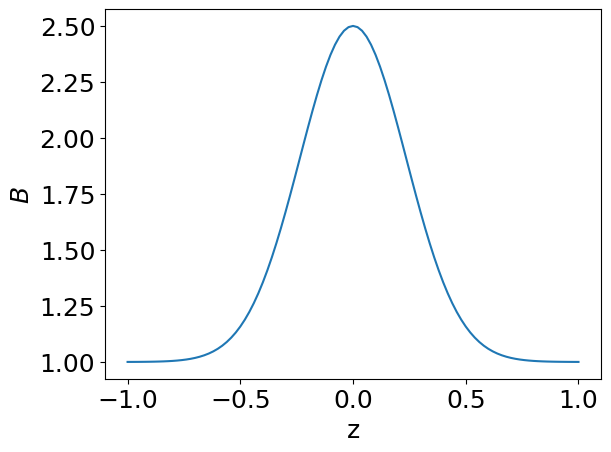
\includegraphics[width=0.7\linewidth]{img/governing-equations/magnetic-field}
	\caption{This is the magnetic field in nozzle with mirror ratio $1+R=B_{max}/B_{min}=2.5$, and the spread of magnetic field, $\delta=0.1/0.3=0.\bar{3}$. }
	\label{fig:magnetic-field}
\end{figure}


\subsection{Velocity Profile at Equilibrium}
Let $n_0$ and $v_0$ be the density and velocity at equilibrium (stationary solution), we know that $\pdv*{n_0}{t}=0$ and $\pdv*{v_0}{t}=0$, therefore $n_0$ and $v_0$ satisfy the so-called equilibrium condition,
\begin{align*}
	&\pdv{z}(\frac{n_0v_0}{B}) = 0 \\
	&v_0\pdv{v_0}{z} = -c_s^2\frac{1}{n_0}\pdv{n_0}{z} 
\end{align*}

Let $M(z) = v_0(z)/c_s$ be the mach number (nondimensionalized velocity). The equations of motion become
\begin{align*}
	&B\pdv{z}(\frac{n_0M}{B}) = 0\\
	&M\pdv{M}{z} = -\frac{1}{n_0}\pdv{n_0}{z}
\end{align*}
Substitute $\frac{1}{n_0}\pdv*{n_0}{z}$ using first equation, the conservation of momentum becomes
\[ (M^2-1)\pdv{M}{z} = -\frac{M}{B}\pdv{B}{z} \]

Notice that there is a singularity at $M=1$, the sonic speed.

This is a separable equation, integrate it and use the conditions at midpoint $B(0)=B_m, M(0)=M_m$ we get
\[ M^2e^{-M^2} = \frac{B^2}{B_m^2}M_m^2e^{-M_m^2} \]
We can now express $M$ using the Lambert W function,
\[ M(z) = \left[ -W_k\left(-\frac{B(z)^2}{B_m^2}M_m^2e^{-M_m^2}\right) \right]^{1/2} \]
where the subscript $k$ of $W$ stands for branch of Lambert W function. When $k=0$, it is the subsonic branch; When $k=-1$, it is the supersonic branch. Below shows a few cases of the solution.
\begin{itemize}
	\item $M_m < 1, k=0$, subsonic velocity profile.
	\item $M_m = 1$, $k=0$ for $x<0$ and $k=-1$ for $x>0$, accelerating profile
	\item $M_m = 1$, $k=-1$ for $x<0$ and $k=0$ for $x>0$, decelerating profile
	\item $M_m > 1, k=-1$, supersonic velocity profile
\end{itemize}
 Fig.(\ref{fig:velocity-profiles}) shows some cases of the solution.
\begin{figure}[H]
	\centering
	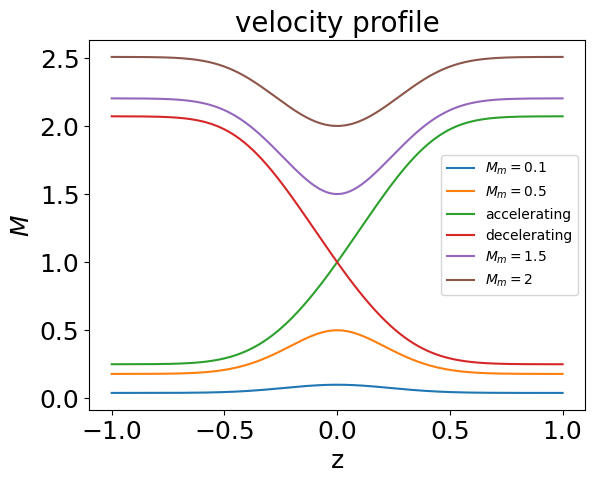
\includegraphics[width=0.7\linewidth]{img/governing-equations/velocity-profiles}
	\caption{The velocity profile in the magnetic nozzle is completely determined by $M_m$, the velocity at the midpoint, $z=0$. For the transonic velocity profiles, $M_m$ alone is not enough to determine the profile, we need to specify the branch of Lambert W function to determine whether it is accelerating or decelerating.}
	\label{fig:velocity-profiles}
\end{figure}



\section{Linearized Equations}
For convenience, we nondimensionalize the governing equations by normalizing the velocity to $c_s$, $v\mapsto v/c_s$, $z$ to system length $L$, $z \mapsto z/L$ and time $t\mapsto c_s t/L$. The governing equations become
\begin{align}
    &\pdv{n}{t} + n\pdv{v}{z} + v\pdv{n}{z} - nv\frac{\partial_z B}{B} = 0 \\
    &n\pdv{v}{t} + nv\pdv{v}{z} = -\pdv{n}{z}
\end{align}
and the nondimensionalized equilibrium condition is
\begin{align}
    &\pdv{z}(\frac{n_0v_0}{B}) = 0 \label{eq:equilibrium-convervation-of-mass}\\
    &v_0\pdv{v_0}{z} = -\frac{1}{n_0}\pdv{n_0}{z} \label{eq:equilibrium-convervation-of-momentum}
\end{align}

Now we are going to derive an important intermediate result, the linearized governing equations.
\begin{proposition}
    Let $n = n_0(z) + \tilde{n}(z,t)$ and $v = v_0(z) + \tilde{v}(z,t)$, where $\tilde{n}$ and $\tilde{v}$ are small perturbed quantities. The linearized governing equations are
    \begin{align}
        &\frac{1}{n_0}\pdv{\tilde{n}}{t} 
        + \pdv{\tilde{v}}{z} + v_0\tilde{Y} + \tilde{v}\frac{\partial_z n_0}{n_0} - \tilde{v}\frac{\partial_z B}{B} = 0 
        \label{eq:linearized-conservation-of-mass}
        \\
        &\pdv{\tilde{v}}{t} + \pdv{(v_0\tilde{v})}{z} = -\tilde{Y}
        \label{eq:linearized-conservation-of-momentum}
    \end{align}
    where 
    \[ \tilde{Y} \equiv \frac{1}{n_0}\pdv{\tilde{n}}{z} - \frac{\partial_z n_0}{n_0^2}\tilde{n} = \pdv{z}(\frac{\tilde{n}}{n_0}) \]
\end{proposition}
\begin{proof}
    We first derive Eq.(\ref{eq:linearized-conservation-of-mass}). We linearize Eq.(\ref{eq:equilibrium-convervation-of-mass}) by setting $n=n_0+\tilde{n}$ and $v=v_0+\tilde{v}$. By ignoring the second order perturbations, we obtain
    \begin{align*}
        &\pdv{(n_0+\tilde{n})}{t} 
        + (n_0+\tilde{n})\pdv{(v_0+\tilde{v})}{z} 
        + (v_0+\tilde{v})\pdv{(n_0+\tilde{n})}{z} 
        - (n_0+\tilde{n})(v_0+\tilde{v})\frac{\partial_z B}{B} = 0 \\
        \Rightarrow 
        &\pdv{\tilde{n}}{t} 
        + n_0\pdv{v_0}{z} + \tilde{n}\pdv{v_0}{z} + n_0\pdv{\tilde{v}}{z}
        + v_0\pdv{n_0}{z} + \tilde{v}\pdv{n_0}{z} + v_0\pdv{\tilde{n}}{z} 
        - (n_0v_0 + n_0\tilde{v} + \tilde{n}v_0)\frac{\partial_z B}{B} = 0 \\
        \Rightarrow
        &\frac{1}{n_0}\pdv{\tilde{n}}{t} 
        + \pdv{v_0}{z} + \frac{\tilde{n}}{n_0}\pdv{v_0}{z} + \pdv{\tilde{v}}{z}
        + \frac{v_0}{n_0}\pdv{n_0}{z} + \frac{\tilde{v}}{n_0}\pdv{n_0}{z} + \frac{v_0}{n_0}\pdv{\tilde{n}}{z} 
        - v_0\frac{\partial_z B}{B} - \tilde{v}\frac{\partial_z B}{B} - \tilde{n}\frac{v_0}{n_0}\frac{\partial_z B}{B} = 0
    \end{align*}
    Using the equilibrium condition Eq.(\ref{eq:equilibrium-convervation-of-mass}), some of the terms are canceled and the last term can be written as 
    \[ \tilde{n}\frac{v_0}{n_0}\frac{\partial_z B}{B} = \frac{\tilde{n}}{n_0}\left( \frac{\partial_z n_0}{n_0}v_0 + \pdv{v_0}{z} \right) \]
    Now, we are left with equation
    \[
        \frac{1}{n_0}\pdv{\tilde{n}}{t}
        + \pdv{\tilde{v}}{z}
        + v_0\underbrace{\left(\frac{1}{n_0}\pdv{\tilde{n}}{z} - \frac{\tilde{n}}{n_0}\frac{\partial_z n_0}{n_0}  \right)}_{\tilde{Y}}
        + \frac{\tilde{v}}{n_0}\pdv{n_0}{z}
        - \tilde{v}\frac{\partial_z B}{B} = 0
    \]

    To derive Eq.(\ref{eq:linearized-conservation-of-momentum}), we linearize the LHS of the conservation of momemtum
    \begin{align*}
        &(n_0+\tilde{n})\pdv{(v_0+\tilde{v})}{t} + (n_0+\tilde{n})(v_0+\tilde{v})\pdv{(v_0+\tilde{v})}{z} = -\pdv{n}{z} \\
        \Rightarrow 
        & \pdv{v_0}{t} + \frac{\tilde{n}}{n_0}\pdv{v_0}{t} + \pdv{\tilde{v}}{t} 
        + \left(v_0+\tilde{v}+\frac{\tilde{n}}{n_0}v_0\right)\pdv{(v_0+\tilde{v})}{z} = -\frac{1}{n_0}\pdv{n}{z}\\
        \Rightarrow
        & \pdv{v_0}{t} + v_0\pdv{v_0}{z} + \tilde{v}\pdv{v_0}{z} 
        = -\frac{1}{n_0}\pdv{n_0}{z} -\frac{1}{n_0}\pdv{\tilde{n}}{z} -v_0\frac{v_0}{z} - \frac{\tilde{n}}{n_0}v_0\pdv{v_0}{z} \\ 
    \end{align*}
    Using the equilibrium condition Eq.(\ref{eq:equilibrium-convervation-of-momentum}) on the RHS, we get the desired form.
\end{proof}


\section{Formulation of the Problem}
In order to investigate the instability of magnetic nozzle, we need formulate it as an eigenvalue problem. To do that, we assume the perturbed density and velocity are oscillatory, i.e. $\tilde{n}, \tilde{v} \sim \exp(-i\omega t)$, where $\omega$ is the oscillation frequency of the perturbed quantities. This frequency can be a complex number. If $\omega = \omega_r +i \omega_i$, then the perturbed quantities becomes $\tilde{n} \sim \exp(\omega_i t)\exp(i\omega_r t)$, which means it grows exponentially with time.

The first step, we can combine Eq.(\ref{eq:linearized-conservation-of-mass}) and Eq.(\ref{eq:linearized-conservation-of-momentum}) into 1 equation.
\begin{proposition}
	\begin{equation}
		\pdv{z}\ln(\frac{n_0}{B}) = -\frac{1}{v_0}\pdv{v_0}{z}
		\label{eq:dv-ln}
	\end{equation}
\end{proposition}
\begin{proof}
	\[ \pdv{z}\ln(\frac{n_0}{B}) 
	= \frac{B}{n_0}\pdv{z}(\frac{n_0}{B})
	= \frac{1}{n_0}\frac{n_0}{z} + B\pdv{z}(\frac{1}{B})
	=
	\frac{1}{n_0}\frac{n_0}{z} \underbrace{- \frac{1}{n_0v_0}\pdv{n_0v_0}{z}}_{Eq.(\ref{eq:equilibrium-convervation-of-mass})}
	= -\frac{1}{v_0}\pdv{v_0}{z} \]
\end{proof}

\begin{proposition}
	Let $\tilde{n}\sim \exp(-i\omega t)$ and $\tilde{v} \sim \exp(-i\omega t)$, then we have the polynomial eigenvalue problem
	\begin{equation}
		\hspace{-0.5in}
		\omega^2 \tilde{v} 
		+ 2i\omega\left(v_0\pdv{}{z} + \pdv{v_0}{z}\right) \tilde{v} 
		+ \left[ (1-v_0^2)\pdv[2]{}{z} 
		-\left(3v_0 + \frac{1}{v_0}\right)\pdv{v_0}{z}\pdv{}{z} 
		- \left(1-\frac{1}{v_0^2}\right)\left(\pdv{v_0}{z}\right)^2 
		- \left(v_0+\frac{1}{v_0}\right)\pdv[2]{v_0}{z} \right]\tilde{v}
		= 0
		\label{eq:polynomial-eigenvalue-problem}
	\end{equation}
\end{proposition}
\begin{proof}
	\begin{align*}
		&\frac{1}{n_0}\pdv{\tilde{n}}{t} 
		+ \pdv{\tilde{v}}{z} + v_0\tilde{Y} + \tilde{v}\frac{\partial_z n_0}{n_0} - \tilde{v}\frac{\partial_z B}{B} = 0 
		\\
		&\pdv{\tilde{v}}{t} + \pdv{(v_0\tilde{v})}{z} = -\tilde{Y}
	\end{align*}
	
	
	We plug Eq.(\ref{eq:linearized-conservation-of-momentum}) in to Eq.(\ref{eq:linearized-conservation-of-mass}), we have 
	\[ -i\omega\frac{\tilde{n}}{n_0} 
	+ \pdv{\tilde{v}}{z} - v_0\left(-i\omega\tilde{v} + \pdv{(v_0\tilde{v})}{z}\right) + \tilde{v}\frac{\partial_z n_0}{n_0} - \tilde{v}\frac{\partial_z B}{B} = 0 \]
	
	Using the equilibrium condition Eq.(\ref{eq:equilibrium-convervation-of-mass}), we can eliminate the term $\partial_z B/B$,
	\begin{align*}
		&-i\omega\frac{\tilde{n}}{n_0} 
		+ \pdv{\tilde{v}}{z} 
		+ v_0\left(i\omega \tilde{v} - v_0\pdv{\tilde{v}}{z} - \tilde{v}\pdv{v_0}{z} \right)
		- \tilde{v}\frac{\partial_z v_0}{v_0} = 0\\
		\Rightarrow
		&-i\omega\frac{\tilde{n}}{n_0} 
		+ i\omega v_0\tilde{v}
		+ (1-v_0^2)\pdv{\tilde{v}}{z} 
		- \left(v_0+\frac{1}{v_0}\right)\pdv{v_0}{z}\tilde{v} = 0
	\end{align*}
	
	Now we take $\pdv*{t}$ on Eq.(\ref{eq:linearized-conservation-of-momentum}). Recall the fact that $\tilde{Y} = \pdv*{(\tilde{n}/n_0)}{z}$, we have
	\begin{align*}
		\omega^2\tilde{v} + i\omega\left(v_0\pdv{\tilde{v}}{z} + \tilde{v}\pdv{v_0}{z}\right) &= \pdv{t}\pdv{z}(\frac{\tilde{n}}{n_0}) \\
		\Rightarrow
		\omega^2\tilde{v} + i\omega\left(v_0\pdv{\tilde{v}}{z} + \tilde{v}\pdv{v_0}{z}\right) &= \pdv{z}(-i\omega v_0\tilde{v}
		- (1-v_0^2)\pdv{\tilde{v}}{z} 
		+ \left(v_0+\frac{1}{v_0}\right)\pdv{v_0}{z}\tilde{v})
	\end{align*}
	Expand the RHS and collect terms, we get
	\begin{align*}
		&\omega^2 \tilde{v} \\ 
		&+2i\omega\left(v_0\pdv{}{z} + \pdv{v_0}{z}\right) \tilde{v} \\ 
		&+\left[ (1-v_0^2)\pdv[2]{}{z} 
		-\left(3v_0 + \frac{1}{v_0}\right)\pdv{v_0}{z}\pdv{}{z} 
		- \left(1-\frac{1}{v_0^2}\right)\left(\pdv{v_0}{z}\right)^2 
		- \left(v_0+\frac{1}{v_0}\right)\pdv[2]{v_0}{z} \right]\tilde{v}
		= 0
	\end{align*}
\end{proof}

Next step we can decouple this equation so that it becomes an eigenvalue problem.
\begin{equation}
	\mqty[ 0 & 1\\ \hat{M} & \hat{N} ]\mqty[ \tilde{v}\\ \omega \tilde{v}] = \omega\mqty[ \tilde{v}\\ \omega \tilde{v}]
	\label{eq:eigenvalue-problem}
\end{equation}
where $O$ is zero matrix, $I$ is identity matrix, and
\begin{align*}
	\hat{M} &= -\left[(1-v_0^2)\pdv[2]{}{z} 
	-\left(3v_0 + \frac{1}{v_0}\right)\pdv{v_0}{z}\pdv{}{z} 
	- \left(1-\frac{1}{v_0^2}\right)\left(\pdv{v_0}{z}\right)^2 
	- \left(v_0+\frac{1}{v_0}\right)\pdv[2]{v_0}{z}\right] \\
	\hat{N} &= -2i\left(v_0\pdv{}{z} +\pdv{v_0}{z} \right) 
\end{align*}
This becomes an algebraic eigenvalue problem if we discretize the operators and the function $\tilde{v}$.




\section{Discretization}

\subsection{Finite Difference}
Using these differentiation matrices, Eq.(\ref{eq:eigenvalue-problem}) becomes
\begin{equation}
	\mqty[ O & I\\ M & N ]\mqty[ \mathbf{\tilde{v}}\\ \omega\mathbf{\tilde{v}} ] = \omega\mqty[ \mathbf{\tilde{v}}\\ \omega\mathbf{\tilde{v}} ]
\end{equation}
where $O$ is a zero matrix, $I$ is an identity matrix, and
\begin{align*}
	M &= -\text{diag}(1-\mathbf{v}_0^2)D^2 
	+\text{diag}\left(3\mathbf{v}_0 + \frac{1}{\mathbf{v}_0}\right) (D\mathbf{v}_0)D 
	+\text{diag}\left(1-\frac{1}{\mathbf{v}_0^2}\right)\left(D\mathbf{v}_0\right)^2 
	+\text{diag}\left(\mathbf{v}_0+\frac{1}{\mathbf{v}_0}\right)(D^2\mathbf{v}_0) \\
	N &= -2i\left(\text{diag}(\mathbf{v}_0)D + D\mathbf{v}_0 \right) 
\end{align*}
Here we abused the notation for the purpose of convenience, $\mathbf{v}_0^2$ means squaring every component of $\mathbf{v}_0$, and $1/\mathbf{v}_0$ denotes 1 divided by all components of $\mathbf{v}_0$.

\subsubsection{Boundary Condition}
We impose Dirichlet boundary condition on the problem, meaning that $\tilde{v}(-1)=\tilde{v}(1)=0$. Further more, the differentiation matrices do not do well on the edges, so during the computation, we remove the first and last row of the differentiation matrices and the vectors $\mathbf{\tilde{v}}$ and $\mathbf{v}_0$. After the computation, we set $\tilde{v}_1=\tilde{v}_N = 0$.


\subsection{Spectral Element}
Suppose the basis functions are $\{u_k(z)\}_{k=1}^\infty$, then the eigenfunction $\tilde{v}$ can be approximated by finite amount of them, $\tilde{v}(z) = \sum_{k=1}^N c_ku_k(z)$ where $c_k$ are coefficients to be determined.

\begin{equation} \label{eq:eigenvalue-problem-SE}
	\mqty[ O & I\\ M & N ]\mqty[ \mathbf{c}\\ \omega\mathbf{c} ] = \omega\mqty[ \mathbf{c}\\ \omega\mathbf{c} ]
\end{equation}
where $O$ is a zero matrix, $I$ is an identity matrix, and
\begin{align*}
	M_{jk} &= -\int_{-1}^{1}dz \; u_{j} \left[(1-v_0^2)\pdv[2]{}{z} 
	-\left(3v_0 + \frac{1}{v_0}\right)\pdv{v_0}{z}\pdv{}{z} 
	- \left(1-\frac{1}{v_0^2}\right)\left(\pdv{v_0}{z}\right)^2 
	- \left(v_0+\frac{1}{v_0}\right)\pdv[2]{v_0}{z}\right] u_{k} \\
	N_{jk} &= -2i\int_{-1}^{1}dz \; u_{j}\left(v_0\pdv{}{z} +\pdv{v_0}{z} \right)u_{k}
\end{align*}

\subsubsection{Boundary Conditions and Basis Function}
To satisfy the Dirichlet boundary condition, $\tilde{v}(\pm 1)=0$, we can choose a set of basis functions that satisfy the boundary condition $u_k(\pm 1)=0,\forall k\in\mathbb{N}$. For example, the sine functions
\[ u_n(z) = \sin(\frac{n\pi}{2}(z+1)), n\in\mathbb{N} \]
is a set of basis functions that satisfy the Dirichlet boundary condition.


\subsection{Finite Element}
Finite-element method is a generalization of the spectral element method. We are allow to use a set of basis functions similar to spectral method in a cell. The region consists of many of these cells.

The formulation is the same as Eq.(\ref{eq:eigenvalue-problem-SE}). The only difference is that in finite-element we need to solve Eq.(\ref{eq:eigenvalue-problem-SE}) simultaneously for all cells.

\subsubsection{Boundary Conditions and B-Spline}
The B-Spline is a commonly used basis function for finite-element method. B-Spline can be defined recursively starting with piecewise constants [reference needed]

\begin{equation}
	B_{i,0}(\xi) = \begin{cases}
		1, &\text{if } \xi_i\leq \xi \leq \xi_{i+1} \\
		0, &\text{otherwise}
	\end{cases}
\end{equation}
For $j\in\mathbb{N}$, they are defined by
\begin{equation}
	B_{i,j}(\xi) = \frac{\xi-\xi_i}{\xi_{i+j}-\xi_i}B_{i,j-1}(\xi) 
	+ \frac{\xi_{i+j+1}-\xi}{\xi_{i+j+1}-\xi_{i+1}}B_{i+1,p-1}(\xi) 
\end{equation}
where $\mathbf{\xi}=[\xi_0,\cdots,\xi_m]$ is called the knot vector, where $m=n+j+1$ where $n+1$ is the number of B-Splines and $j$ is the degree of B-Spline polynomials. The knot vector defines the shapes of the B-Splines, see Fig.\ref{fig:bspline}. The variable $\xi$ is within the range $[\xi_0, \xi_m]$. 

Any function $u(x)$ on $[\xi_0,\xi_N]$ can be approximated by
\[ u(x) \simeq \sum_{j=0}^{n} c_jB_{i,j}(x) \]

The Dirichlet boundary condition can be set by letting the coefficients of the first and last B-Spline to 0, $c_{0}=c_{n} = 0$, where $N$ is the number of B-Splines.


\begin{figure} [H]
	\centering
	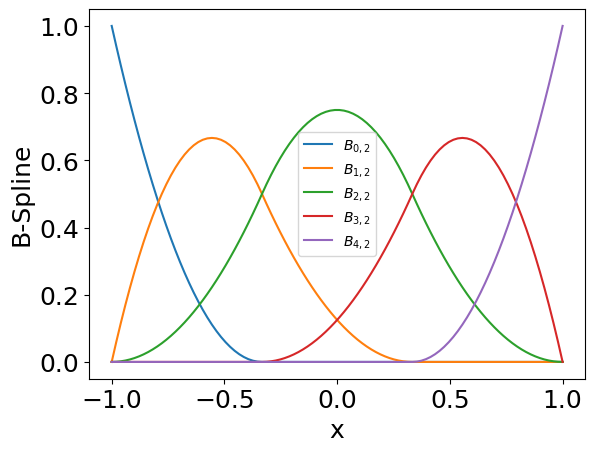
\includegraphics[width=0.7\linewidth]{img/governing-equations/bspline}
	\caption{An example of open uniform quadratic B-Spline on $[-1,1]$. The knot vector is $[-1,-1,-1,-1/3,1/3,1,1,1]$.}
	\label{fig:bspline}
\end{figure}

